% =====================================================================================================
\section{Protocol and Defence Evaluation}\label{sec:protocol}
\textit{Setup.} Sender, network channel, receiver and logger run as separate processes that talk over UDP, so the evaluation exercises the real wire format, fragmentation and timing. The sender encodes 320$\times$240 video at 10 frames/s with the golden model (the same bytes as the RTL), fragments every frame into datagrams of at most 1400 bytes and sends them; the channel can impose loss, delay, jitter and reordering and implements the attacker of Section~\ref{sec:threat}. All runs used a 4-core cloud virtual machine; the same scripts run against the board (Section~\ref{sec:board}).

\textit{Active attacks.} The full scenario applies \NumAttacks{} attacks for six seconds each, 25\,s apart: bit flips in the scan, a mode downgrade in the header, splicing of two frames, injection of a forged frame, replay, delay, dropping, a junk flood, and dropping, forging and replaying feedback. Table~\ref{tab:attacks} gives the result over \SuiteRuns{} runs. Every attack was mitigated in every run, on average \TtmMean{}\,$\pm$\,\TtmSd{}\,s after it began, with \SuiteFalse{} false alarms in calm windows and a median frame latency of \SuiteLatency\,ms. The slowest case, dropped feedback, is caught only by the dead-man rule, after about \FbDropTtm\,s: the 3\,s timeout plus part of a decision window. With a trailer, a talking-head clip or Tears of Steel as the video source instead of the synthetic scene, all attacks were again mitigated (\RealTrailerMit{}, \RealTalkMit{} and \RealOpenMit{}; means \RealTrailerTtm{}, \RealTalkTtm{} and \RealOpenTtm{}\,s, one run each) without false alarms.

% generated by paper/make_assets.py from paper/data -- do not edit
\begin{table}[t]
\caption{Reaction to each active attack (full suite, threshold policy, 3 runs; mean\,$\pm$\,s.d. in seconds). ``First rejection'' is when the receiver first discards a frame; ``mitigated'' is when the sender has raised protection or rekeyed.}
\label{tab:attacks}
\centering\small\setlength{\tabcolsep}{4pt}
\resizebox{\columnwidth}{!}{%
\begin{tabular}{lccc}
\toprule
Attack & Mitigated & First rejection & Mitigated after \\
\midrule
bit flips in the scan & 3/3 & 0.09\,$\pm$\,0.03 & 0.41\,$\pm$\,0.02 \\
mode downgrade in header & 3/3 & 0.06\,$\pm$\,0.02 & 0.44\,$\pm$\,0.02 \\
splice of two frames & 3/3 & 0.13\,$\pm$\,0.00 & 0.46\,$\pm$\,0.01 \\
forged frame injection & 3/3 & 0.14\,$\pm$\,0.06 & 0.44\,$\pm$\,0.03 \\
frame replay & 3/3 & 0.07\,$\pm$\,0.05 & 0.46\,$\pm$\,0.03 \\
frame delay & 3/3 & 4.13\,$\pm$\,0.04 & 1.46\,$\pm$\,0.03 \\
frame dropping & 3/3 & -- & 1.46\,$\pm$\,0.03 \\
junk flood & 3/3 & -- & 0.49\,$\pm$\,0.04 \\
feedback dropping & 3/3 & -- & 3.47\,$\pm$\,0.05 \\
forged feedback & 3/3 & -- & 0.46\,$\pm$\,0.04 \\
feedback replay & 3/3 & -- & 0.44\,$\pm$\,0.01 \\
\bottomrule
\end{tabular}}
\end{table}


\begin{figure*}[t]
\centering
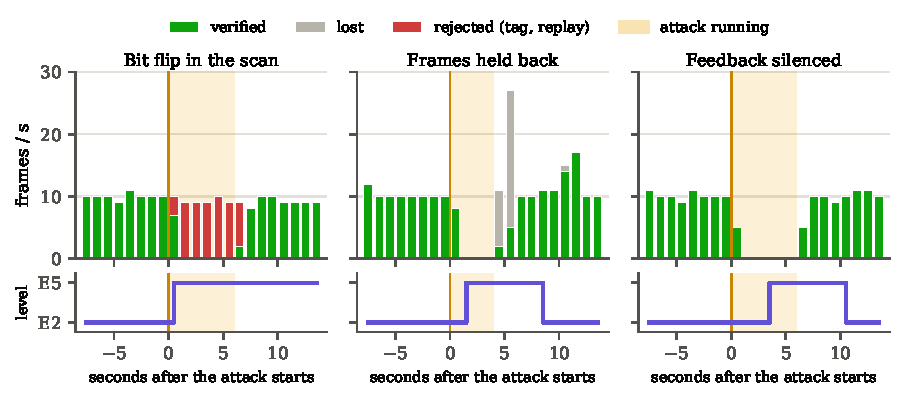
\includegraphics[width=0.92\textwidth]{figures/fig_case_evidence.pdf}
\caption{Three attacks as the sender sees them (one full-suite run): frames per second from the receiver's authenticated heartbeats, and the protection level. A bit flip fails the tag at once; held-back frames produce no rejection while the attack lasts and return as a gap of lost frames; silenced feedback leaves the receiver's video intact but blinds the sender until the dead-man rule fires.}
\label{fig:caseevidence}
\end{figure*}

\textit{The evidence decides the reaction time.} The attacks of Table~\ref{tab:attacks} are all mitigated, but Fig.~\ref{fig:caseevidence} shows that they leave three different kinds of evidence, and the evidence, not the harm, sets how fast the defence can react. A bit flip is the easy case: the receiver rejects the first tampered frame after \CaseBitflipFirstRej\,s on average over \CaseRuns{} runs and the sender reaches E5 after \CaseBitflipAware\,s. Holding frames back produces no rejection while it lasts, because nothing arrives at all. When the next frame gets through, the receiver counts the gap as lost frames; the held frames, released after the \CaseDelayDuration\,s attack, still carry valid tags but are older than frames already shown, so they are discarded as late (\CaseDelayRejected{} per run, the first \CaseDelayFirstRej\,s after the attack began), the verdict our replay window gives to benign reordering. The defence therefore never sees a delay: it reacts after \CaseDelayAware\,s to video that stops while heartbeats still arrive, which it treats as jamming. Silencing the feedback path is the mirror image. The receiver sees perfect video and rejects \CaseFbdropRejected{} frames, yet the sender, which learns about the link only through authenticated heartbeats, goes blind, and only the dead-man rule escalates, after \CaseFbdropAware\,s. The stream stays at its floor level longest during this attack, which gives it the highest leakage of all attacks while active (\CaseFbdropLeak, the mean edge correlation of the active level). Integrity attacks are caught at the first frame; attacks by absence can only be caught by a timeout, so their reaction time is a design parameter, and shortening it trades against false alarms on a slow network.

\textit{Benign impairments.} A second scenario applies only network problems: rising packet loss up to 6\,\%, delay up to 120\,ms with jitter, and 5\,\% reordering. Over \BenignRuns{} runs the defence raised no false alarm (\BenignFalse{} windows); median latency was \BenignLatency\,ms and the 95th percentile \BenignPninetyfive\,ms. This needed loss to be judged over three windows and late frames to be told apart from replays.

\begin{figure}[t]
\centering
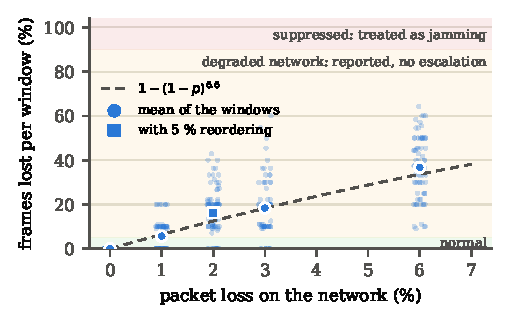
\includegraphics[width=\columnwidth]{figures/fig_case_loss.pdf}
\caption{Frame loss against packet loss in the benign scenario (\BenignRuns{} runs; small dots: one-second windows, large: means). The dashed curve is~\eqref{eq:fragloss}, fitted to the points without reordering. The shading is the policy's classification of frame loss.}
\label{fig:caseloss}
\end{figure}
\textit{A third of the frames lost, and no alarm.} A frame of $n$ fragments is lost when any fragment is, so with independent packet loss $p$
\begin{equation}
P_{\mathrm{frame}} = 1 - (1 - p)^n \approx n p \quad (np \ll 1).
\label{eq:fragloss}
\end{equation}
Fig.~\ref{fig:caseloss} shows how badly a lossy network treats a fragmented video stream: at \CaseSixPct\,\% packet loss the receiver lost \CaseSixFrameLoss\,\% of the frames, \CaseAmplification{} times the packet loss, and the points without reordering follow~\eqref{eq:fragloss} with $n \approx \CaseFragments$ fragments per frame. Even so, the defence did not escalate once, because loss between 5 and 90\,\% is reported as a degraded network; the highest threat score~\eqref{eq:threat} of any benign window was \CaseBenignMaxThreat, half the level at which Table~\ref{tab:attacks} counts the sender as aware. The same rule is a limitation: jamming that lets more than a tenth of the frames through is indistinguishable from a bad network. Forward error correction across fragments would lower the curve, at a bitrate cost.

\textit{Threshold rule against bandit.} The learning scenario repeats a bit-flip and a replay attack five times each, separated by calm periods. We ran both policies with \Seeds{} paired seeds (Table~\ref{tab:policies}, Fig.~\ref{fig:policies}). The result is a consistent trade-off rather than a winner. The bandit encrypted fewer bits in every seed (\PolCostB{} against \PolCostT{} of the payload, \PolCostSave\,\% less), but it reacted later (\PolTtmB{} against \PolTtmT\,s) and leaked more while attacks were active (\PolLeakB{} against almost zero), again in every seed. Neither policy raised a false alarm (\PolFalse{}). The reason is the loss~\eqref{eq:loss}: the bandit pays for encrypted bits in every calm window and for leakage only in the windows after an attack is visible, so it learns to sit lower and climb when evidence appears. We keep the threshold rule as the default; the bandit suits links where bandwidth matters more than the first second of an attack.

% generated by paper/make_assets.py from paper/data -- do not edit
\begin{table}[t]
\caption{Threshold rule vs.\ $\varepsilon$-greedy bandit on the learning scenario, 10 seeds each (mean\,$\pm$\,s.d.). The last column counts the seeds in which the bandit was better (lower) than the threshold rule with the same seed.}
\label{tab:policies}
\centering\small\setlength{\tabcolsep}{4pt}
\resizebox{\columnwidth}{!}{%
\begin{tabular}{lccc}
\toprule
Metric & Threshold & Bandit & Bandit better \\
\midrule
Mitigation (s) & 0.46\,$\pm$\,0.02 & 1.34\,$\pm$\,0.03 & 0/10 \\
Leakage under attack & 0.000\,$\pm$\,0.001 & 0.054\,$\pm$\,0.004 & 0/10 \\
Encrypted share & 0.188\,$\pm$\,0.001 & 0.162\,$\pm$\,0.001 & 10/10 \\
Encrypted share, calm & 0.135\,$\pm$\,0.000 & 0.138\,$\pm$\,0.001 & 0/10 \\
\bottomrule
\end{tabular}}
\end{table}

\begin{figure}[t]
\centering
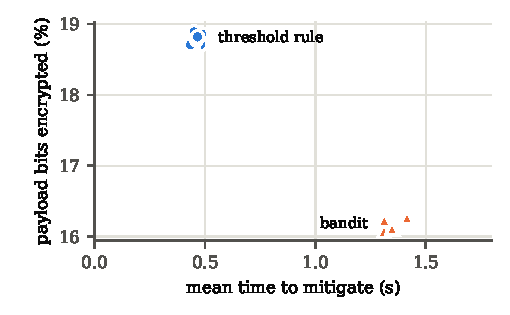
\includegraphics[width=\columnwidth]{figures/fig_policies.pdf}
\caption{Encrypted share of the payload against mean time to mitigate, one point per seed and policy (\Seeds{} paired seeds).}
\label{fig:policies}
\end{figure}

\textit{Cost relative to software.} On the simulation host, our Python model needs \PyPlainMs\,ms to encode a 640$\times$480 frame and \PySelEtwoMs\,ms including E2 selective encryption, whereas libjpeg-turbo takes \TurboMs\,ms and full-stream AES-GCM about \AesGcmMs\,ms. A desktop processor is the wrong baseline; what matters is the SoC's ARM core, which has no AES instructions (Section~\ref{sec:board}).
